\documentclass[12pt]{article}
\usepackage{graphicx,multicol,mdwlist}
\usepackage{charter,amsmath,amssymb,breakurl}
\usepackage{eulervm}
\usepackage[letterpaper,margin=1in]{geometry}
\title{Math 265 Quiz 4}\author{}\date{}
\let\cos\relax\DeclareMathOperator{\cos}{\mathsf{cos}}
\let\ln\relax\DeclareMathOperator{\ln}{\mathsf{ln}}
\everymath{\displaystyle}
\begin{document}
\maketitle
\thispagestyle{empty}
\begin{multicols}{2}
Consider the vector field $\mathbold{F}\left(x,y\right)
=\left\langle y-y^2,x-xy\right\rangle$, which is shown
at the right, together with the cardioid $C$
given by $r=2-2\sin{\theta}$.
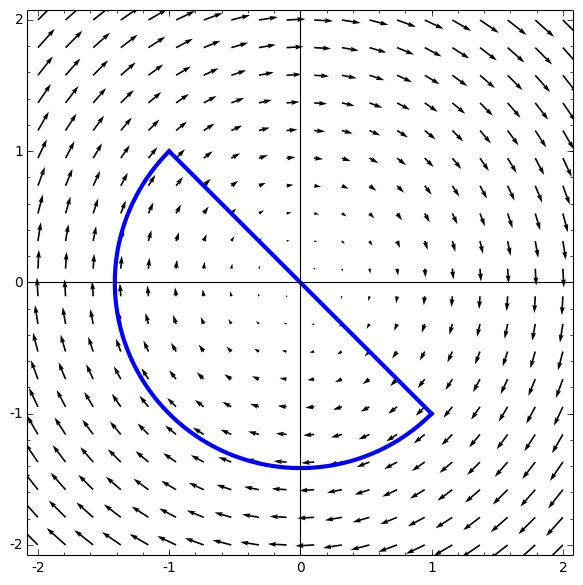
\includegraphics[scale=.5]{Cardioid}
\end{multicols}
\begin{enumerate}
\item\label{FirstConservative} Is $\mathbold{F}$ conservative?
\item Calculate the outward flux $\oint_C\mathbold{F}
\cdot\mathbold{n}\;ds$ using Green's Theorem.
\item Calculate the line integral $\int_D\mathbold{F}
\cdot d\mathbold{r}$ using a method of your choice,
where $D$ is the arc of $C$ with $0\le t\le\frac{\pi}{2}$.
\end{enumerate}
\end{document}
